\documentclass[11pt]{article}
\usepackage{amsmath}
\usepackage{amssymb}
\usepackage{graphicx}
\usepackage{geometry}[0.9in]
\usepackage{url}

\renewcommand{\vec}[1]{\boldsymbol{#1}}
\newcommand{\hvec}[1]{\hat{\vec{#1}}}

\title{Clarifications on scattering factors and scattering densities.}
\author{Richard Kirian}
\date{\today}
\begin{document} 

\maketitle

\section{Objective}

We sometimes wish to construct a scattering density for an ensemble of atoms so that we may use a fast Fourier transform method to generate scattering amplitudes.  However, it is usually the atomic form factors and dispersion corrections that are found in the literature (because this is what can be measured).  Here we wish to determine the effective scattering densities from available tables.

\section{Atomic scattering density and atomic scattering factor}



Far-field x-ray diffraction intensities under the first Born approximation are equal to 
\begin{align}\label{eqn:qrf}
I(\vec{q}) = J_0 \Delta \Omega r_e^2 P \left| \sum_n^N f_n(q) \exp(-i \vec{q}\cdot\vec{r}_n)\right|^2
\end{align}
where $J_0$ is the incident photon fluence (photons per area), $\Delta \Omega$ is the solid angle of the detector pixel (assumed to be small), $r_e$ is the classical electron radius, $P$ is the polarization factor that depends on the beam polarization, the incident wavevector $\vec{k}_\text{in}$, and the outgoing wavevector $\vec{k}_\text{in}$, $f_n(q)$ is the atomic scattering factor (assumed rotationally symmetric), $\vec{r}_n$ is the position vector of the $n$th atom, and the wavevector transfer is $\vec{q} = \vec{k}_\text{out}-\vec{k}_\text{in}$.  We may define a continuum of complex scattering density $\rho(\vec{r})$ such that
\begin{align}\label{eqn:dft}
I(\vec{q}) = J_0 \Delta \Omega r_e^2 P(\hvec{q},\hvec{b}) \left| \int \rho(\vec{r}) \exp(-i \vec{q}\cdot\vec{r}) \; d^3r\right|^2 \; .
\end{align}

If we consider just a single rotationally symmetric atom situated at the origin, the atomic form factor is equal to
\begin{align}
f(q)  &= \int \rho(r) \exp(-i \vec{q}\cdot\vec{r}) \; d^3r \\
  &= \int_0^\infty \rho(r)   \frac{\sin(qr)}{qr}  4\pi r^2 dr \; . \label{eqn:form}
\end{align}
For an atom located at the position $\vec{r}_n$ we have
\begin{align}
%f(\vec{q})  &= \int \rho(|\vec{r}-\vec{r}_n|) \exp(-i \vec{q}\cdot\vec{r}) \; d^3r \\
%  &= \exp(-i \vec{q}\cdot\vec{r}_n) \int \rho(|\vec{r}-\vec{r}_n|) \exp(-i \vec{q}\cdot (\vec{r}-\vec{r}_n)) \; d^3r \\
f(\vec{q})  &= f(q)\exp(-i \vec{q}\cdot\vec{r}_n)  \; .
\end{align}
We may take the inverse Fourier transforms to arrive at %the expression for the scattering density in terms of the atomic scattering factor:
\begin{align}
\rho(r)  &= (2\pi)^{-3} \int  f(q)  \exp(i \vec{q}\cdot\vec{r}) \; d^3q \\
&= (2\pi)^{-3} \int_0^\infty f(q)   \frac{\sin(qr)}{qr}  4\pi q^2 dq \; . \label{rhor}
\end{align}
If we are well above resonances, $\rho(\vec{r})$ is well approximated as the electron number density.    Atomic scattering factors are often approximated by a $q$-dependent ``atomic form factor'' $f_0(q)$  that is related to the Fourier transform of the electron density, along with a complex energy-dependent (but $q$-independent) ``anomalous dispersion correction'' $\Delta f(E) =  f'(E) + i f''(E)$: 
\begin{align}
f(q) = f_0(q) + \Delta f(E) = f_0(q) + f'(E) + i f''(E)  \;.
\end{align}
Plugging these in we have
\begin{align}
\rho(r)  &= (2\pi)^{-3} \int  (f_0(q) + \Delta f(E))   \exp(i \vec{q}\cdot\vec{r}) \; d^3q \\
&=  \delta(\vec{r}) \Delta f(E) + (2\pi)^{-3} \int_0^\infty f_0(q)    \frac{\sin(qr)}{qr}  4\pi q^2 dq  \\
&=  \delta(\vec{r}) \Delta f(E) + \rho_0(r) \; .
\end{align}
For an atom at position $\vec{r}_n$ we have
\begin{align}
\rho_n(\vec{r})  &=  \delta(\vec{r}-\vec{r}_n) \Delta f_n(E) + \rho_{0n}(|\vec{r}-\vec{r}_n|) \; .
\end{align}
In order to build our complete scattering density we take the sum
\begin{align}
\rho(\vec{r})  &= \sum_n \delta(\vec{r}-\vec{r}_n) \Delta f_n(E) + \rho_{0n}(|\vec{r}-\vec{r}_n|) \; .
\end{align}
Our chores are to (1) figure out a way to programmatically access the needed scattering factors in order to build a scattering density sampled about a 3D grid, (2) decide on how to lay out delta functions in the typical situation in which the atoms do not lie exactly on grid points, (3) do the transforms in equation \ref{rhor} numerically and perhaps tabulate the results, and (4) find a means to efficiently place the resulting $\rho(\vec{r})$ densities into a 3D grid.


%It is a simple matter to use equation \ref{eqn:qrf}, except that we need to have a programmatic way to look up the scattering factors $f_n(\vec{q})$.  One objective here is to establish how to do this in Python.  The Fourier transform needed in equation \ref{eqn:dft} is also straightforward in principle with a standard fast fourier transform (FFT), except that we must keep in mind that the FFT inherently returns the intensities corresponding to a periodic object, we need to calculate $\rho(r)$ from the tabulated scattering factors $f(q)$, and we need to construct a density map with attention to the sampling of the atomic densities.  In particular, the scattering factors $f(q)$ have constant terms due to anomalous dispersion corrections, which are complex delta functions in real space.  Delta functions are in principle impossible to sample on a finite grid (unless they are centered exactly at a grid point).

\section{Hubbel form factors}

Hubbel {\itshape et al.} (1975)\cite{hubbellAtomicFormFactors1975} have provided tables of atomic form factors that are still in widespread use today.  They provide atomic form factors $F(q,Z)$ (atomic number $Z$) that are defined exactly as in equation \ref{eqn:form}.
%They define the following:
%\begin{align}
%\rho(\vec{r}) = (2\pi)^{-3} \int F(\vec{q},Z) \exp(i\vec{q}\cdot\vec{r}) d^3q
%\end{align}
%and the tabulated values are the form factors
%\begin{align}
%F(q,Z) = 4\pi \int_0^\infty \rho(r) \frac{\sin(qr)}{qr} r^2 dr \;.
%\end{align}
The form factors $F(q,Z)$ are accessible programatically from the  \texttt{xraylib} library, which has a Python wrapper.

\section{Henke dispersion corrections}
Henke {\itshape et al.}\cite{henkeXRayInteractionsPhotoabsorption1993} have compiled experimental dispersion corrections that appear to be among the best available.  The Henke tables are largely meant for soft-x-ray work and as such they do not include $q$-dependent scattering factors.
%Their diffraction formula is
%\begin{align}
%A=-A_0 \frac{r_0}{r} P(\phi) f
%\end{align}
%where $A$ is the scattered amplitude and $A_0$ is the incident amplitude, $r_0$ is the classical electron radius, $r$ is the far-field distance, $P(\phi)$ is a polarization correction, and 
In the Henke {\itshape et al.}\cite{henkeXRayInteractionsPhotoabsorption1993} notation, the scattering factor is defined as
\begin{align}
f=f_1+if_2=f_1(0)-\Delta f_0(\theta)+if_2(0)
\end{align}
and is related to the index of refraction by
\begin{align}
n_r = 1 - \delta -i\beta = 1 -\frac{r_0\lambda^2}{2\pi}\sum_q n_qf_q(0) \; .
\end{align}
The refractive index is always related to the electron density according to
\begin{align}
\rho =  \frac{2\pi}{\lambda^2 r_0 } \left( 1 - n_r \right) = \frac{2\pi}{\lambda^2 r_0 } \left( \delta + i \beta \right) 
\end{align}
The tabulated values of $f_1$ and $f_2$ are available in gzip format at the CXRO website \url{http://henke.lbl.gov/optical_constants/asf.html}).  The \texttt{bornagain} package provides programmatic access to them.


\section{xraylib}

The \texttt{xraylib} library\cite{schoonjansXraylibLibraryXray2011,brunettiLibraryXrayMatter2004} provides access to the atomic form factors  $F(x,Z)$  from Hubbel {\itshape et al.}\cite{hubbellAtomicFormFactors1975}.  They are accessed through the function \texttt{FF\_Rayl(Z,q)} -- one can easily confirm correspondence with the Hubbel tables.  The dispersion corrections are also accessible through the functions \texttt{Fi(Z,E)} and \texttt{Fii(Z,E)}, but there is no mathematical definition of these functions in the \texttt{xraylib} publications, nor is there an explanation of where they come from.   Empirically, the $f$ defined in the Henke tables is nearly equal to the quantity $\texttt{FF\_Rayl(Z,q)} + \texttt{Fi(Z,E)} - i\; \texttt{Fii(Z,E)}$ that can be constructed from \texttt{xraylib}.  Note the unconventional negative sign in front of the \texttt{Fii(Z,E)} term.  Figure \ref{fig:forms} shows plots comparing the tabulated Henke tables and \texttt{xraylib} functions, which shows near equality, but the Henke tables seem to have greater resolution near resonances.
\begin{figure}[htbp]
   \centering
   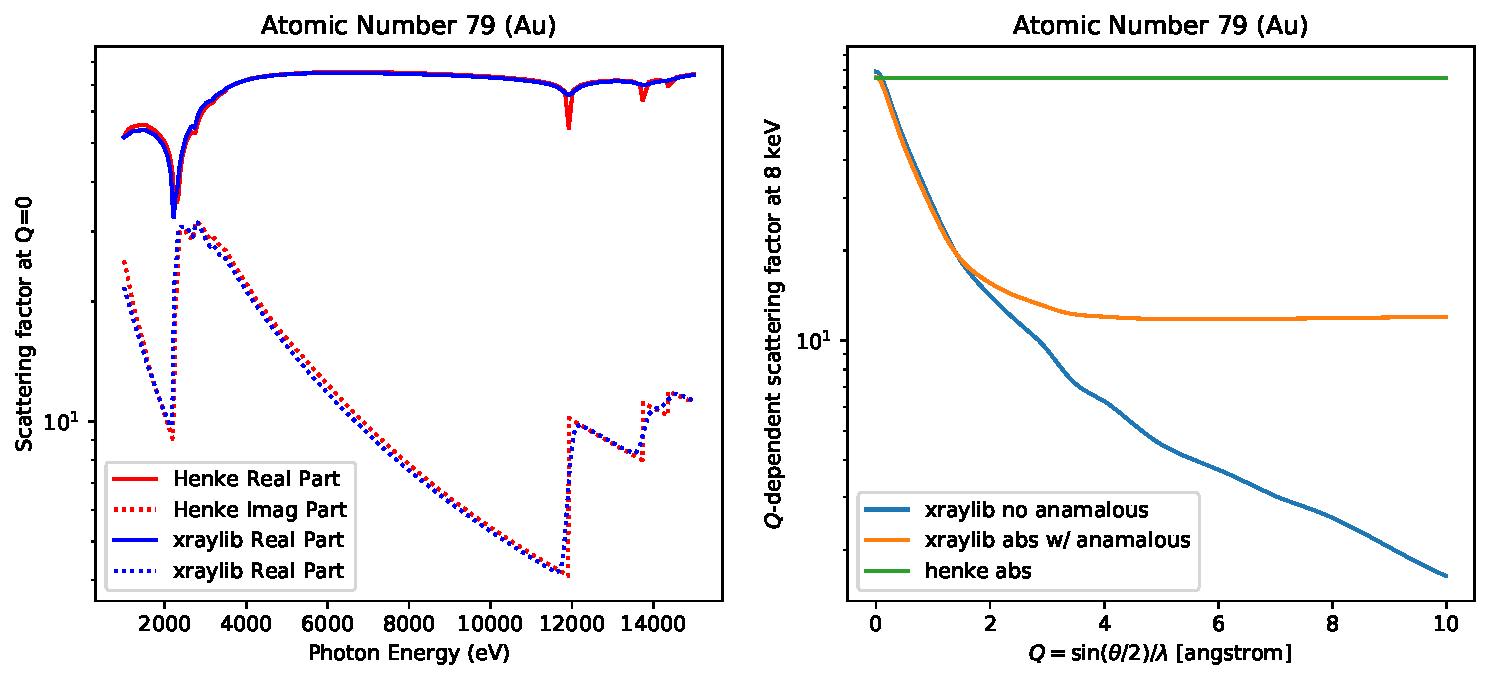
\includegraphics[width=\textwidth]{formfactor_79.pdf} 
   \caption{Energy-dependent form factor in the forward scattering direction and the $Q$-dependent form factor.  Comparison between Henke tables and \texttt{xraylib} for gold.  The plots were generated with the file \texttt{developer/rkirian/misc/scattering\_factors.py}.}
   \label{fig:forms}
\end{figure}


%which give the anomalous scattering factors $\phi'$ and $\phi''$.  The differential Rayleigh cross section for unpolarized light is defined as:
%\begin{align}
%\frac{d\sigma_R}{d\Omega} = \frac{r_e^2}{2}(1+\cos^2\theta)F^2(x, Z)
%\end{align}
%where $x = \sin(\theta/2)/\lambda$ and 
%The anomalous factors appear only in the equations:
%\begin{align}
%n &= 1- \delta -i \beta \\
%\delta &= \frac{h^2 e^2}{E^2 2\pi m_e} \sum_a \frac{N_A}{A} \rho \phi_a' \\
%\beta &= \frac{h^2 e^2}{E^2 2\pi m_e} \sum_a \frac{N_A}{A} \rho \phi_a''
%\end{align}
%Using the relation $E = hc/\lambda$ and the classical electron radius $r_e = e^2/m_ec^2$ we can write
%\begin{align}
%n &= 1-  \frac{e^2}{c^2 2\pi m_e} \lambda^2 \sum_a \frac{N_A}{A} \rho (\phi_a' + i \phi_a'') \\
%\end{align}

\section{bornagain}

These Henke scattering factors (at $q=0$) are returned as a single complex number $f$ from the function \texttt{get\_scattering\_factors(Z,E)}, which is in the \texttt{bornagain.simulate.atoms} sub-module.  \texttt{bornagain} also has wrappers to the xraylib functions for convenience since they use different units and they are not vectorized functions (hence they are very slow).  The combined Hubbel form factors and Henke dispersion corrections may be accessed through the function \texttt{bornagain.simulate.atoms.hubbel\_henke\_atomic\_form\_factors}.




\section{Getting to the density}

We are provided with $F(q)$ and the relation 
\begin{align}
\rho(r) = (2\pi)^{-3} \int F(q) \exp(i\vec{q}\cdot\vec{r}) d^3q = (2\pi)^{-3} \int_0^{2\pi}d\phi \int_{-1}^1 d\cos\theta \int_0^\infty q^2 dq F(q) \exp(i\vec{q}\cdot\vec{r})
\end{align}
Since $F(q)$ and $\rho(r)$ are spherically symmetric, we are free to choose $\vec{r}$ along the $z$ axis so that $\vec{q}\cdot\vec{r} = qr \cos\theta$.  We then do the integral as follows:
\begin{align}
%\rho(r) &= (2\pi)^{-3} \int_0^{2\pi}d\phi \int_0^\infty q^2 dq  F(q) \int_{-1}^1 d\cos\theta  \exp(iqr\cos\theta) \\
%&= (2\pi)^{-2}  \int_0^\infty q^2 dq  F(q)  \frac{1}{iqr}\int_{-iqr}^{iqr} dx  \exp(x) \\
%&= (2\pi)^{-2}  \int_0^\infty q^2 dq  F(q)  \frac{2\sin(qr)}{qr} \\
%&= 2(2\pi)^{-2}\frac{1}{r}  \int_0^\infty  dq   [q F(q)]  \sin(qr) \\
2 \pi^2 r \rho(r) &=  \int_0^\infty  dq   [q F(q)]  \sin(qr)  \label{eqn:trans}
\end{align}
We wish to do the above quickly using a numpy FFT function.  In numpy, the inverse DFT is defined in the following way:
\begin{align}\label{eqn:idft}
a_n = \frac{1}{N}\sum_{k=0}^{N-1}A_k\exp\left(2\pi i{nk\over N}\right) \qquad n = 0,\ldots,N-1
\end{align}
Let's define the following:
\begin{align}
\rho_m &= 2 \pi^2 m\Delta r \rho(m \Delta r) \\
F_k &= k \Delta q F(k \Delta q)
\end{align}
By taking a discrete integral with samples in $q$ we have an approximation for equation \ref{eqn:trans}:
\begin{align}
2 \pi^2 r \rho(r) &\approx  \sum_{k=0}^{N-1}  \Delta q   [k \Delta q F(k \Delta q)]  \sin(k \Delta q r)  \\
  &\approx  \text{Im} \left\{ \sum_{k=0}^{N-1}  \Delta q   [k \Delta q F(k \Delta q)]  \exp( i k \Delta q r) \right\}
\end{align}
Next we take discrete samples in $r$:
\begin{align}\label{eqn:almostft}
2 \pi^2 n \Delta r \rho(n \Delta r) &\approx  \text{Im} \left\{ \sum_{k=0}^{N-1}  \Delta q   [k \Delta q F(k \Delta q)]  \exp( i k \Delta q n \Delta r) \right\}
\end{align}
We know what values we need for $\Delta r$ and $r_\text{max} = N \Delta r$.  Looking at the argument in the exponential of equations \ref{eqn:idft} and \ref{eqn:almostft} we see that we should define our $q$-space increment $\Delta q  = 2\pi / \Delta r N$ so that
\begin{align}
\pi n \Delta r^2 \rho(n \Delta r) &\approx  \text{Im} \left\{ \frac{1}{N}  \sum_{k=0}^{N-1}     [k \Delta q F(k \Delta q)]  \exp\left( 2\pi i \frac{nk}{ N} \right) \right\}
\end{align}
Finally we define 
\begin{align}
F_k &= k \Delta q F(k \Delta q)
\end{align}
so that
\begin{align}
\rho(n \Delta r) &\approx \frac{1}{\pi n \Delta r^2 } \text{Im} \left\{ \frac{1}{N}  \sum_{k=0}^{N-1}    F_k  \exp\left( 2\pi i \frac{nk}{ N} \right) \right\}
\end{align}
%f_n &= 2 \pi^2 n \Delta r \rho(n \Delta r) 


\section{Appendix}

\subsection{Fourier transform of rotationally symmetric object}

If we consider just a single atom situated at the origin, the atomic form factor is equal to
\begin{align}
 f(\vec{q})  = \int \rho(r) \exp(-i \vec{q}\cdot\vec{r}) \; d^3r \; .
\end{align}
Due to rotational symmetry, we are free to choose a convenient direction $\vec{q} = q \hvec{z}$ such that in the spherical coordinate system we have $\vec{q}\cdot\vec{r} =  q r \cos\theta$.  Now we write down our Fourier transform with reference only to the magnitudes $q$ and $r$:
\begin{align}
f(\vec{q})  &= \int_0^{2\pi} d\phi \int_0^\infty \rho(r) r^2 dr \int_0^\pi \sin\theta d\theta  \exp(-i q r \cos\theta)  \\
&=2\pi \int_0^\infty \rho(r) r^2 dr \int_{-1}^1  d\cos\theta  \exp(-i q r \cos\theta)  \\
&=2\pi \int_0^\infty \rho(r) r^2 dr \frac{1}{-iqr}\int_{iqr}^{-iqr}  du  \exp(u)  \\
&=2\pi \int_0^\infty \rho(r) r^2 dr \frac{\exp(iqr) - \exp(-iqr)}{iqr}   \\
f(q) &= \int_0^\infty \rho(r)   \frac{\sin(qr)}{qr}  4\pi r^2 dr  
\end{align}


\newpage




\bibliography{\jobname}
\bibliographystyle{plain}

\end{document}
